\documentclass{ximera}

\graphicspath{  
{./}
{./whoAreYou/}
{./drawingWithTheTurtle/}
{./bisectionMethod/}
{./circles/}
{./anglesAndRightTriangles/}
{./lawOfSines/}
{./lawOfCosines/}
{./plotter/}
{./staircases/}
{./pitch/}
{./qualityControl/}
{./symmetry/}
{./nGonBlock/}
}


%% page layout
\usepackage[cm,headings]{fullpage}
\raggedright
\setlength\headheight{13.6pt}


%% fonts
\usepackage{euler}

\usepackage{FiraMono}
\renewcommand\familydefault{\ttdefault} 
\usepackage[defaultmathsizes]{mathastext}
\usepackage[htt]{hyphenat}

\usepackage[T1]{fontenc}
\usepackage[scaled=1]{FiraSans}

%\usepackage{wedn}
\usepackage{pbsi} %% Answer font


\usepackage{cancel} %% strike through in pitch/pitch.tex


%% \usepackage{ulem} %% 
%% \renewcommand{\ULthickness}{2pt}% changes underline thickness

\tikzset{>=stealth}

\usepackage{adjustbox}

\setcounter{titlenumber}{-1}

%% journal style
\makeatletter
\newcommand\journalstyle{%
  \def\activitystyle{activity-chapter}
  \def\maketitle{%
    \addtocounter{titlenumber}{1}%
                {\flushleft\small\sffamily\bfseries\@pretitle\par\vspace{-1.5em}}%
                {\flushleft\LARGE\sffamily\bfseries\thetitlenumber\hspace{1em}\@title \par }%
                {\vskip .6em\noindent\textit\theabstract\setcounter{question}{0}\setcounter{sectiontitlenumber}{0}}%
                    \par\vspace{2em}
                    \phantomsection\addcontentsline{toc}{section}{\thetitlenumber\hspace{1em}\textbf{\@title}}%
                     }}
\makeatother



%% thm like environments
\let\question\relax
\let\endquestion\relax

\newtheoremstyle{QuestionStyle}{\topsep}{\topsep}%%% space between body and thm
		{}                      %%% Thm body font
		{}                              %%% Indent amount (empty = no indent)
		{\bfseries}            %%% Thm head font
		{)}                              %%% Punctuation after thm head
		{ }                           %%% Space after thm head
		{\thmnumber{#2}\thmnote{ \bfseries(#3)}}%%% Thm head spec
\theoremstyle{QuestionStyle}
\newtheorem{question}{}



\let\freeResponse\relax
\let\endfreeResponse\relax

%% \newtheoremstyle{ResponseStyle}{\topsep}{\topsep}%%% space between body and thm
%% 		{\wedn\bfseries}                      %%% Thm body font
%% 		{}                              %%% Indent amount (empty = no indent)
%% 		{\wedn\bfseries}            %%% Thm head font
%% 		{}                              %%% Punctuation after thm head
%% 		{3ex}                           %%% Space after thm head
%% 		{\underline{\underline{\thmname{#1}}}}%%% Thm head spec
%% \theoremstyle{ResponseStyle}

\usepackage[tikz]{mdframed}
\mdfdefinestyle{ResponseStyle}{leftmargin=1cm,linecolor=black,roundcorner=5pt,
, font=\bsifamily,}%font=\wedn\bfseries\upshape,}


\ifhandout
\NewEnviron{freeResponse}{}
\else
%\newtheorem{freeResponse}{Response:}
\newenvironment{freeResponse}{\begin{mdframed}[style=ResponseStyle]}{\end{mdframed}}
\fi



%% attempting to automate outcomes.

%% \newwrite\outcomefile
%%   \immediate\openout\outcomefile=\jobname.oc
%% \renewcommand{\outcome}[1]{\edef\theoutcomes{\theoutcomes #1~}%
%% \immediate\write\outcomefile{\unexpanded{\outcome}{#1}}}

%% \newcommand{\outcomelist}{\begin{itemize}\theoutcomes\end{itemize}}

%% \NewEnviron{listOutcomes}{\small\sffamily
%% After answering the following questions, students should be able to:
%% \begin{itemize}
%% \BODY
%% \end{itemize}
%% }
\usepackage[tikz]{mdframed}
\mdfdefinestyle{OutcomeStyle}{leftmargin=2cm,rightmargin=2cm,linecolor=black,roundcorner=5pt,
, font=\small\sffamily,}%font=\wedn\bfseries\upshape,}
\newenvironment{listOutcomes}{\begin{mdframed}[style=OutcomeStyle]After answering the following questions, students should be able to:\begin{itemize}}{\end{itemize}\end{mdframed}}



%% my commands

\newcommand{\snap}{{\bfseries\itshape\textsf{Snap!}}}
\newcommand{\flavor}{\link[\snap]{https://snap.berkeley.edu/}}
\newcommand{\mooculus}{\textsf{\textbf{MOOC}\textnormal{\textsf{ULUS}}}}


\usepackage{tkz-euclide}
\tikzstyle geometryDiagrams=[rounded corners=.5pt,ultra thick,color=black]
\colorlet{penColor}{black} % Color of a curve in a plot



\ifhandout\newcommand{\mynewpage}{\newpage}\else\newcommand{\mynewpage}{}\fi


\title{What is a matrix?}

\outcome{View points as column matrices.}
\outcome{View a matrix as a function.}
\outcome{Compute the product of a $3\times 3$ matrix and a $1\times 3$ matrix.}
\outcome{Explain what an isometry is.}
\outcome{Use the distance formula to compute the distance between two points.}

\author{Jenny Sheldon \and Bart Snapp}

\begin{document}
\begin{abstract}
  We will think of a matrix as a function.
\end{abstract}
\maketitle

We're going to discuss some basic functions in geometry.
Specifically, we will talk about translations, reflections, and
rotations. To start us off, we need a little background on
\textit{matrices}.\index{matrix} You might think of a matrix as just a jumble
of large brackets and numbers:
\[
\begin{bmatrix}
  2 & 3 & -4 & 8 \\
  -2 & 8 & 9 & -1 \\
  0 & 4 & 9 & -7\\
  1 & 0  & -3 & 9
\end{bmatrix}
\]
However, we are going to think of
matrices as \textit{functions}. Just as we write $f(x)$ for a function
$f$ acting on a number $x$, we'll write:
\[
\mat{M} \vec{p} = \vec{q} 
\]
to represent a matrix $\mat{M}$ mapping point $\vec{p}$ to point
$\vec{q}$. A point $\vec p$ is often represented as an ordered pair of
coordinates, $\vec{p} = (x,y)$. However, to make things work out
nicely, we need to write our points all straight and narrow, with a
little buddy at the end:
\[
(x,y) \leadsto \begin{bmatrix} 
x \\ 
y \\
1
\end{bmatrix}
\]
Throughout this chapter, we will abuse notation slightly, freely
interchanging several notations for a point:
\[
\vec{p} \leftrightsquigarrow
(x,y) \leftrightsquigarrow
\begin{bmatrix} 
x \\ 
y \\
1
\end{bmatrix}
\]
With this in mind, our work will be done via matrices and
points that look like this:
\[
\mat{M} = 
\begin{bmatrix}
a & b & c \\ 
d & e & f \\
0 & 0 & 1
\end{bmatrix}\qquad\text{and}\qquad \vec{p} = 
\begin{bmatrix}
x \\
y \\
1
\end{bmatrix}
\]
Now recall the nitty gritty details of \textit{matrix
  multiplication}:\index{matrix!multiplication}
\begin{align*}
\mat{M} \vec{p} &= 
\begin{bmatrix}
a & b & c \\ 
d & e & f \\
0 & 0 & 1
\end{bmatrix}
\begin{bmatrix}
x \\
y \\
1
\end{bmatrix} \\
&= \begin{bmatrix}
ax + by + c\cdot 1\\
dx + ey + f\cdot 1\\
0\cdot x + 0 \cdot y  + 1\cdot 1
\end{bmatrix}\\
&= \begin{bmatrix}
ax + by + c\\ 
dx + ey + f\\
1
\end{bmatrix}
\end{align*}

Try you hand at this.
\begin{question}
  Compute:
  \[
  \begin{bmatrix}
    -9 & 1 & 3 \\ 
    6 & -4 & -4 \\
    0 & 0 & 1
  \end{bmatrix}
  \begin{bmatrix}
    5 \\
    6 \\
    1
  \end{bmatrix}
  \]
  \begin{prompt}
    Write with me:
    \begin{align*}
      \begin{bmatrix}
    -9 & 1 & 3 \\ 
    6 & -4 & -4 \\
    0 & 0 & 1
  \end{bmatrix}
  \begin{bmatrix}
    5 \\
    6 \\
    1
  \end{bmatrix} &=
    \begin{bmatrix}
    -45 +\answer{6} +3 \\
    \answer{30}-24 -4 \\
    1
    \end{bmatrix}\\
    &=  \begin{bmatrix}
    \answer{-36} \\
    \answer{2} \\
    1
  \end{bmatrix}
    \end{align*}
  \end{prompt}
\end{question}


\begin{question} Fine, but what does this have to do with geometry?

Maybe this video will help:
  \begin{center}
  \youtube{vQ60rFwh2ig}
\end{center}
\end{question}

In this chapter we are going to study a special type of functions,
called \textit{isometries}. These are functions that preserve
distances. Let's see what we mean by this:

\begin{definition} 
An \dfn{isometry} is a function $\mat{M}$ that maps points in the
plane to other points in the plane such that
\[
d(\vec{p}, \vec{q}) = d(\mat{M} \vec{p},\mat{M}\vec{q}),
\]
where $d$ is the distance function.
\end{definition}


\begin{question}
  How do you compute the distance between two points again?
  \begin{multipleChoice}
    \choice[correct]{I remember how to do this.}
    \choice[correct]{I don't remember how to do this.}
  \end{multipleChoice}
  \begin{question}
    If needed check out: \link[Euclidean distance]{https://en.wikipedia.org/wiki/Euclidean_distance}


    
    Check your understanding by computing the distance between:
    \[
    \vec{p}= (1,3) \quad\text{and}\quad\vec{q}(2,4)
    \]
    \begin{prompt}
      \[
      d(\vec{p},\vec{q}) = \answer{\sqrt{2}}
      \]
    \end{prompt}
  \end{question}
\end{question}

%% \begin{question} IDENTIFY ISOMETRY FROM PHOTO
%% Now consider this photo that was taken by \link[Christian Mehlf\"uhrer]{https://en.wikipedia.org/wiki/File:MC_Drei-Finger-Faultier.jpg}
%% \begin{image}
%%   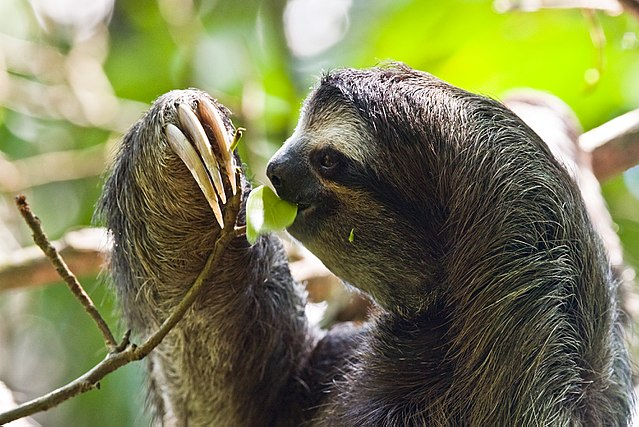
\includegraphics{sloth.jpg}
%% \end{image}
%% Below we see several transformed vers
%% \end{question}

We're going to see that several ideas in geometry which all seem very different are actually all isometries.  Specifically, we'll look at
translations, reflections, and rotations.  Since they are isometries, 
we will be thinking of these concepts as matrices.

\end{document}
